\def\year{2016}
%File: formatting-instruction.tex
\documentclass[letterpaper]{article}
\usepackage[ruled,vlined,linesnumbered]{algorithm2e}
\usepackage{aaai}
\usepackage{times}
\usepackage{helvet}
\usepackage{color}
\usepackage{graphicx}
\usepackage{courier}
\usepackage{amsthm}
\usepackage{amsmath}
\usepackage[round]{natbib}
\usepackage{url}

\newcommand\note[1]{\textcolor{red}{#1}}

\frenchspacing
\setlength{\pdfpagewidth}{8.5in}
\setlength{\pdfpageheight}{11in}



\pdfinfo{
/Title (Privacy Preserving LAMA)
/Author (Submission \#19)}
\setcounter{secnumdepth}{0}  

\newtheorem{definition}{Definition}
\newtheorem{theorem}{Theorem}
\newcommand\roni[1]{\textcolor{blue}{roni: #1}}
\newcommand\guy[1]{\textcolor{red}{guy: #1}}

\theoremstyle{definition}
\newtheorem{example}{Example}[section]


\setcounter{secnumdepth}{2}

 \begin{document}
% The file aaai.sty is the style file for AAAI Press 
% proceedings, working notes, and technical reports.
%
\title{Privacy Preserving LAMA}
\author{\#?}
%}
\maketitle
\begin{abstract}
\begin{quote}
Privacy-preserving multi-agent planning (PP-MAP) is a recently introduced setting 
in which agents collaborate to achieve a goal but each agent may keep some facts it knows about the world private. A prominent approach in the development of PP-MAP algorithms is to use various components from single agent planning algorithms and adapt them so that privacy is preserved. In this short paper we show how the components of LAMA, arguably one of the most successful single-agent planners, can be used in a privacy preserving manner. These components include a landmark heuristic, an FF heuristic, preferred operators and deferred node evaluation. These components are integrated into the Greedy Privacy Preserving Planner (GPPP), a state-of-the-art PP-MAP algorithm. The resulting algorithm performs better than other PP-MAP algorithms from the recent Competition of Distributed and Multiagent Planners. 
\end{quote}
\end{abstract}


\section{Introduction}

% Motivation: PP-MAP is so great
In certain cases, several agents may cooperate to achieve joint goals, while concealing certain facts concerning their abilities. Take for example an army organization outsourcing its food supply to external caterers. The caterers and the army operate jointly to provide food to the army bases. On the other hand, the army may not want the location of these bases, or the number of soldiers on each base to be disclosed to the caterers. The caterer may not wish the army to be aware of the number of trucks it operates. One approach to concealing these private facts is by using logistics centers, where the caterer unloads packaged food, and the army trucks then deliver the packages to the various bases. The army and the caterer must plan together to deliver appropriate amounts of food to the various logistic centers at the right time, while not disclosing the number and location of the bases, as well as the number of trucks.


% We use the MA-STRIPS formalism. It is so popular everyone should work only on it
\cite{brafman2013complexity} proposed an attractive framework for such planning problems called multi-agent STRIPS (MA-STRIPS). Indeed, MA-STRIPS attracted much attention in recent years~\cite{tozicak2015onInternally,torreno2015global,vstolba2014relaxation,maliah2014privacyPreserving}. The first Competition of Distributed and Multiagent Planners (CoDMAP), held last year, already featured many planners from 10 different groups.

%there has even been a recent Competition of Distributed and Multiagent Planners (CoDMAP) which featured many MA-STRIPS planners from 10 different groups. 

% Still, single agent planners are much stronger, so much work on borrowing ideas from there
Many successful privacy preserving MA-STRIPS planning algorithms borrow or adapt algorithmic components from the single-agent planning literature. For example, privacy preserving versions have been proposed for popular single-agent heuristics such as landmarks~\cite{maliah2014privacyPreserving,torreno2015global,vstolba2015admissible}, FF~\cite{vstolba2014relaxation}, and pattern databases~\cite{maliah2015privacy}. 


LAMA is, arguable, one of the most successful single-agent planner to-date. In this short paper we integrate various components of LAMA into the Greedy Privacy Preserving Planner (GPPP)~\cite{maliah2014privacyPreserving}. The resulting privacy preserving planner is called PP-LAMA. Some of the components of PP-LAMA were already introduced in previous work, while other components are novel. Specifically, PP-LAMA has the following LAMA-based improvement over GPPP: (1) an improved privacy preserving landmark detection algorithm able to find all landmarks as in the single agent case, (2) alternating this heuristic with a privacy preserving version of  FF introduced by \cite{vstolba2014relaxation}, (3) used preferred operators and deferred node evaluation. 

The contribution of this work is three-fold. First, in the improved landmark detection algorithm. Second, a privacy preserving way to implement preferred operators and lazy node geneartion. Third, we integrate all this improvements into PP-LAMA and show that it outperforms all other planners over the CoDMAP problems. In addition, we observe that the deferred heuristic lazy evaluation of LAMA is especially useful for the time consuming collaborative effort in computing the privacy preserving FF heuristic.


%method heuristic in the adaption of preferred operators  describe a better landmark

%adaptation of various components of LAMA into a privacy preserving setting and integrate them in a single, highly effective, privacy preserving planner. Specifically, we focus on the following LAMA components:

%the landmark computation mechanism, the FF heuristic, and preferred operators. Our landmark identification improves upon previously suggested privacy preserving landmark identification approaches, obtaining the same set of landmarks as LAMA would identify when ignoring the privacy constraints. The deferred heuristic lazy evaluation of LAMA is especially useful for the time consuming collaborative effort in computing the privacy preserving FF heuristic.




%In an effort to take advantage of the success of single agent planning algorithms, various algorithmic components of 

%A popular and successful approach is based on forward heuristic search~\citep{nissim2014distributed,maliah2015privacy,maliah2014privacyPreserving,vstolba2014relaxation,vstolba2015admissible}. Several  heuristics have been suggested for this task, including an adaptation of the FF heuristic \citep{vstolba2015admissible} and landmarks \citep{maliah2014privacyPreserving}. 

%In classical planning it is widely agreed that landmarks --- logic formulas that must occur on every path to goal --- provide a good, yet partial, estimate for the distance to the goal \citep{richter2008landmarks}. Indeed, landmarks are typically combined with other heuristics in order to achieve a competitive performance in heuristic search. Specifically, the LAMA planner \citep{richter2010lama} combines landmarks with the FF heuristic \citep{hoffmann2001ff} to achieve an impressive performance on classical planning benchmark domains.

%In this short paper we provide an adaptation of LAMA into a privacy preserving setting, which we call PP-LAMA. We explain the various components of PP-LAMA --- the landmark computation mechanism, the FF heuristic, and preferred operators. Our landmark identification improves upon previously suggested privacy preserving landmark identification approaches, obtaining the same set of landmarks as LAMA would identify when ignoring the privacy constraints. The deferred heuristic lazy evaluation of LAMA is especially useful for the time consuming collaborative effort in computing the privacy preserving FF heuristic.

%We provide experiments on benchmarks form the latest CoDMAP competition, showing PP-LAMA to solve more problems than any other privacy preserving planner.

\section{Background}

We now briefly describe the privacy preserving planning setting, the LAMA algorithm, and the classical landmark identification and FF heuristics.

\subsection{Privacy Preserving Planning}

\begin{figure}
\centering
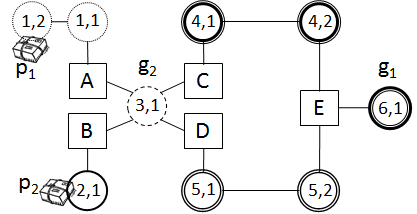
\includegraphics[scale=0.7]{Logistics}
\label{fig:logistics}
%\caption{A logistics example, where trucks deliver packages between logistics centers, denoted by squares. Each agent covers a set of cities, denoted by circles, and labeled $i,j$ where $i$ is the agent covering the city and $j$ is the local city index. The logistic centers can be entered by several agents, serving as collaboration sites.}
\caption{A logistics example.}
\end{figure}

An MA-STRIPS problem\citep{brafman2013complexity} is represented by a tuple $\langle V, \{A_i\}_{i=1}^k, I ,G \rangle$ where:
\begin{itemize}
	\item $k$ is the number of agents
%	\item $V$ is a finite set of finite-domain variables. 
	\item $P$ is a finite set of facts (can be true of false). 
%    \item For $1\leq i \leq k$, $A_i$ is the set of actions agent $i$ can perform. 
    \item $A_i$ is the set of actions agent $i$ can perform. 
	\item $I$ is the start state.
	\item $G$ is the goal condition.	
\end{itemize} 

Each action $a=\langle pre(a), eff(a) \rangle$ is defined by its preconditions ($pre(a)$), and effects ($eff(a)$). Preconditions and effects are logical formulas of $P$. A state is a conjunction of facts in $P$ (true or false). The goal $G$ is a also a conjunction of facts. The result of applying an action $a$ to a state $s$ is denoted by $a(s)$. A solution to a planning task is a {\em plan} $\pi=(a_1,\ldots,a_k)$ such that $G\subseteq a_k(\ldots(a_1(I)\ldots)$, i.e., a sequence of actions that transforms the initial state ($I$) to a state satisfying the goal condition ($G$). 

Privacy-preserving MA-STRIPS extends MA-STRIPS by defining sets of variables and actions as private, known only to a single agent. To define this notion of privacy more generally, let $public(P)$ be the set of public facts in $P$. Let $public_i(A) \subset A_i$ be the set of public actions of agent $i$. When a public action is executed, all agents are aware of the execution, and view the public effects of the action.
Let $private_i(P)$ and $private_i(A)$ denotes the variables and actions that are private to agent $i$, respectively. For ease of exposition we assume that all goals are public.

A solution to a privacy-preserving MA problem, is a sequence of public and private actions. We say that the sequence of public actions in such a solution is a high-level, or public, plan, that must be extended to a full plan using private actions of various agents. Given a valid high-level plan each agent can plan independently to achieve the preconditions on the public actions it executes in the high level plan \citep{maliah2014privacyPreserving}.

Figure~\ref{fig:logistics} illustrates a simple logistic example in which the agents are trucks tasked with delivering packages. 

The set of facts $P$ represents the location of the two packages and six trucks. Each truck has three actions: move, load, and unload, corresponding to moving the truck between locations, loading a package and unloading it. Trucks can only drive along the edges in Figure~\ref{fig:logistics}. Agents are heterogeneous  and their range is restricted, such that location $i,j$ can only be reached using truck $i$. The rectangles are logistic centers visited by multiple trucks that load or unload packages. 

Each truck is owned by a different company, and one company does not want to share its location and coverage (which locations it can reach) with other companies. Thus, all the facts representing the location of trucks are private, while the facts representing whether a package is at a logistic center are public. Only the load/unload actions at the logistic centers are public, where the move actions are private for each agent, as well as loading and unloading packages at private locations.  


\subsection{LAMA}

LAMA is a classical planning algorithm, which has repeatedly demonstrated strong pref romance in planning competitions \citep{richter2010lama}. Due to the lack of space, we provide here a very brief review of LAMA, avoiding many details. LAMA uses heuristic search, with two different heuristics --- landmarks and the FF heuristic. The heuristics are maintained in 4 separate open lists, and the search alternates in selecting which node to expand from the lists.

Landmarks are propositional formulas that must be satisfied during the execution of every successful plan \citep{richter2008landmarks}. A popular method for identifying landmarks, searches backwards from the goal. At each phase, one landmark is selected for development. All actions that can satisfy this landmarks are identified, and a new landmark is constructed from their preconditions. When all these actions share a single fact, that fact is identified as a new landmark. Otherwise, a disjunctive formula is created from some facts that appear in the actions preconditions. When developing a landmark, all actions that take facts in this landmark as preconditions are ignored, in order to avoid circular reasoning.

The FF heuristic begins by computing the relaxed planning graph, where facts are organized into layers, and all edges are between consecutive layers \citep{hoffmann2001ff}. The first layer contains all the facts that hold at the current search state. Given a layer, the next layer is constructed by executing all actions whose precondition is satisfied by the facts in the current layer. Then, all the facts in these action effects are added to the next layer, ignoring delete effects. Once an action has participated in the construction of a layer, it is not considered again. For each fact $p$ we maintain the action $a_p$ that has achieved it for the first time. Then, we construct an edge between the preconditions of $a_p$ on the previous level and $p$.

After the graph construction, FF computes a plan over the relaxed graph, starting from the goal and moving backwards. First, we consider the goal facts, and add all the actions that achieved them to the plan, then we consider the preconditions of these actions, and so forth, ignoring repeated facts.

\subsection{GPPP}

The GPPP algorithm \citep{maliah2014privacyPreserving} is a heuristic best-first privacy preserving planner. The algorithm begins by searching for a high level public plan. The algorithm maintains a global queue of states to expand, where each state is represented by the set of public facts that hold for that state, and a set of private state identifiers, one for each agent. Every agent can map its private identifiers to a set of private facts.

GPPP uses only public actions to expand the current state. Every time a state is expanded, all agents participate in computing the expanded state. Each agent estimates using delete relaxation which private facts it can achieve following the public action execution, and which public actions can now be executed given these private facts. 


In addition, agents collaborate in computing a heuristic value for the expanded state. For example, in a landmark heuristic, each agent reports the number of landmarks that are satisfied in that state. Although GPPP has shown impressive coverage, the need to collaborate for evaluating the heuristic of each expanded state slows down the search process considerably.

After each state expansion, all agents report whether they can reach all goals given the expanded states. As GPPP estimates states using delete relaxation, even if the agents report that all goals can be achieved, the public plan that achieves them may not be sound. Thus, once a public plan has been achieved, the agents compute private plans to achieve the preconditions of the public actions in the high level plan. If this phase fails, because some agent cannot achieve the preconditions of a public action, then the high level search continues.

Our PP-LAMA algorithm builds upon GPPP. The main changes in PP-LAMA are the use of multiple queues, and the lazy heuristic estimation.

\section{Privacy Preserving Heuristics}

In this section we describe PP-LAMA --- a privacy preserving LAMA implementation. We begin by describing the privacy preserving landmark identification mechanism, and then the privacy preserving FF heuristic computation. Finally we describe the privacy preserving LAMA algorithm itself.

\subsection{Privacy Preserving Landmark Computation}

We use the landmark identification heuristic of \citep{maliah2014privacyPreserving}, where agents collaborate in identifying landmarks, and augment it with an improved detection for private landmarks. The process begins with all agents agreeing on a landmark to develop. This landmark can be a public fact, a private fact, or a disjunction of public and private facts. All agents then compute iteratively the set of public facts that can be achieved, avoiding actions that have the landmark facts as preconditions, to avoid circular reasoning.

Then, using the published set of public facts, all agent develop the landmark backwards, obtaining a new landmark. Each agent develops its own private parts of the landmark, and all agents develop together the public parts of the landmark.
This landmark, again, can be composed of public and private facts. Only the public facts are published to the other agents. For private facts, all agents agree on a unique ID for this landmark, and each agent maintains a mapping from this ID to its own set of private facts that participate in this landmark. 

Our landmark identification phases improves upon the original LM-GPPP by allowing us to identify and develop landmarks that contain private facts of multiple agents. LM-GPPP allowed only for landmarks with private facts of a single agent.

During execution time, when evaluating a state, each agent published which landmarks it can satisfy in this state. Then, we globally count the number of landmarks that at least one agent can satisfy, and this is used as the landmarks heuristic estimate for that state.

\subsection{Privacy Preserving FF}

We use the privacy preserving ff heuristic computation suggested by \citep{vstolba2015admissible}. The method constructs the relaxed planning graph jointly, with each agent maintaining only a part of the graph, using its own actions. After each agent computes its own next level of achievable facts, the public facts in that level are published to the other agents, and all agents insert these public facts into their local current layer. When a public fact has been achieved for the first time by several agents at the same level, one agent is considered to be responsible for achieving it, and the fact is labeled by the public action that this agent has used to achieve the fact.

The construction of the relaxed plan is also done in collaboration, where each agent computes a part of the plan, containing its own actions. Agents may use an action in the plan that requires a precondition fact that was generated by another agent. That agent is then notified to continue constructing the plan to achieve the precondition. When the plan construction phase has terminated, all agents report the number of actions in their portion of the relaxed plan. The sum of these counts is the FF heuristic estimate for that state.

\subsection{Preferred Operators}

A preferred operator is an action that is deemed to be valuable at a given state. These are computed differently for the FF heuristic and for the landmark heuristic.

The FF heuristic computes a relaxed plan, distributed between the agents. All agents are aware, though, of the public actions in this relaxed plan and their order. The computation of the preferred operators is based on this public subset of the relaxed plan.

For FF heuristic, the preferred operators are actions that achieve at least one public precondition of a public action in the relaxed plan. For the landmark heuristic, the preferred operators are actions that appear prior to the first landmark that the relaxed plan achieves.


\section{Privacy Preserving LAMA}

We now describe the implementation of the privacy preserving LAMA algorithm --- PP-LAMA. We employ a best first search for a high level public plan, developing at each step the most promising state, given the heuristic value. We maintain 4 separate open lists sorted on all the heuristics above --- FF, landmarks, FF preferred operators, and landmarks preferred operators.


PP-LAMA is described in Algorithm~\ref{alg:PP-LAMA}. The best first search chooses which open list to use at each step, giving priority to the preferred operator open lists (line 25), and alternating between landmarks and FF. Once a state was chosen, PP-LAMA computes heuristic values for this state. This is a lazy heuristic evaluation, as opposed to GPPP that computes heuristic values for every expanded state, and is designed to reduce the number of costly heuristic computation messages.

Then, PP-LAMA expands the state using all applicable public actions, and inserts all the expanded states with the heuristic value of their parent. This is known as deferred heuristic evaluation \citet{richter2010lama}. 

\begin{algorithm}[t!]
\footnotesize
	\SetKwBlock{PPLAMA}{PP-LAMA()}{end}
\PPLAMA{
	%\KwIn{$\pi_i$, the local view of agent $i$}
  	%\KwOut{$P_{full}$, a complete plan} 
    
    Init all open lists to hold the initial state\\
    $c_{preferred} \leftarrow 1$\\
    $c_{\overline{preferred}} \leftarrow 0$\\
    $turn \leftarrow 1$\\
   
    \While{some open list is not empty}{
		\If{$c_{preferred} > c_{\overline{preferred}}$}{
        	\If{$turn=0$}{
            	{\em active-list}$\leftarrow$ preferred landmark open list\\
            }
            \Else{
            	{\em active-list}$\leftarrow$ preferred FF open list\\
            }
        }
        \Else{
        	\If{$turn=0$}{
            	{\em active-list}$\leftarrow$ landmark open list\\
            }
            \Else{
            	{\em active-list}$\leftarrow$ FF open list\\
            }
        }
        $s \leftarrow $ best state in {\em active-list}\\
        Remove $s$ from all open lists\\
        $turn \leftarrow (turn+1) \% 2$\\
        \If{$s \models G$}{
        	$P_{pub}\leftarrow $ the public plan to achieve $s$\\
        	$P_{full}\leftarrow$ private extensions for $P_{pub}$\\
            \If{$P_{full}$ is valid}{
            	\Return $P_{full}$\\
            }
        }
        Compute all heuristic values for $s$\\
        \If{$c_{preferred} > c_{\overline{preferred}}$ and $s$ has the best heuristic value thus far}{
        	$c_{preferred} \leftarrow c_{preferred} + 1000$\\
        }
        \Else{
        	$c_{\overline{preferred}} \leftarrow c_{\overline{preferred}} + 1$\\
        }
        \ForEach{public action $a_{pub}$ applicable in $s$}{
            $s' \leftarrow apply(s, a_{pub})$
            \If{$a_{pub}$ is a preferred operator for $s$}{
                Insert $s'$ into all open lists, with the heuristic value of $s$\\
            }
            \Else{
                Insert $s'$ into the landmarks and FF open lists, with the heuristic value of $s$\\
            }
        }    
    }


}
\caption{The PP-LAMA algorithm} 
\label{alg:PP-LAMA}
\end{algorithm}


\section{Empirical Evaluation}

We evaluate the performance of PP-LAMA over all benchmarks from the CoDMAP competition. We compare PP-LAMA to all relevant algorithms from the competition. All experiments were run on a 2.67 GHz machine with 32GB of memory running Windows. All algorithms were implemented in C\#.

We first compute the coverage of PP-LAMA, comparing it to other relevant planners from the latest CoDMAP \citep{vstolba2015competition}. As Table~\ref{tbl:codmap} shows, PP-LAMA solves the most problem instances overall. In addition, on all but two domains, it is the best performing planner.



\begin{table}[t]
\scriptsize
\centering
\begin{tabular}{l|rrrrrr}

Domain			&GPPP	&MAPR	&PMR	&MAPlan/ &PSM-	&PP-		\\
	    		&		&-p	    &	    &FF+DTG	 &VRD	&LAMA 		\\\hline
blocksworld		&12		&20		&20		&20		&20		&20			\\
depot			&11		&0		&0		&13		&17		&18			\\
driverlog		&14		&20		&19		&17		&20		&20			\\
elevators		&20		&19		&19		&11		&12		&20			\\
logistics		&20		&19		&0		&18		&18		&20			\\
rovers			&19		&19		&20		&20		&12		&20			\\
satellites		&18		&20		&19		&20		&18		&20			\\
sokoban			&9		&0		&6		&18		&18		&12			\\
taxi			&20		&0		&19		&20		&0		&20			\\
wireless		&3		&2		&7		&4		&0		&4			\\
woodworking		&18		&0		&0		&16		&19		&19			\\
zenotravel		&20		&20		&18		&20		&13		&20			\\	\hline
total			&184	&139	&147	&197	&167	&213		\\

\end{tabular}
\caption{Coverage results for a timeout of 30 minutes over the CoDMAP instances.}
\label{tbl:codmap}
\end{table}


To better understand the advantage of PP-LAMA over other algorithms that employ either the FF heuristic \citep{vstolba2015admissible} and landmarks \citep{maliah2014privacyPreserving}, we analyze the performance of the search mechanism when using only some of the heuristics. Table~\ref{tbl:heuristics} presents experiments when using only the FF heuristic, only landmarks, both the FF and the landmark heuristics using alternating lists without the lazy evaluation, and the complete PP-LAMA. We report both coverage, and average time for obtaining a solution over domains that all variants were able to solve.

Clearly, FF is both the slowest heuristic to compute, and also produces the poorest results when executed alone. Landmarks are faster to compute, as they are identified only once, and then the agents only need to evaluate which landmarks are satisfied in the current state, rather than compute a relaxed plan, as done for FF. The combination of both landmarks and FF is somewhat better, but the largest gain comes from the overall LAMA approach, and mostly from the lazy deferred heuristics and the preferred operators. PP-LAMA, although it uses the FF heuristic, is very fast, because the heuristics are computed only for states that are removed from the open list, not for all generated states.


\begin{table}[t]
\scriptsize
\centering
\begin{tabular}{|l||r|r||r|r||r|r||r|r|}
\hline
			&\multicolumn{2}{c|}{FF}&\multicolumn{2}{c||}{landmarks}&\multicolumn{2}{c||}{FF+landmarks}&\multicolumn{2}{c|}{LAMA} 		\\ 
Domain&C&T&C&T&C&T&C&T \\ \hline\hline
blocksworld	&18	&49	&12	&36	&20	&49	&20	&12	\\ \hline
depot	&3	&25	&11	&19	&10	&22	&18	&1	\\ \hline
driverlog	&14	&155	&14	&203	&17	&27	&20	&3	\\ \hline
elevators	&20	&148	&20	&25	&20	&149	&20	&4	\\ \hline
logistics	&20	&8	&20	&2	&20	&8	&20	&1	\\ \hline
rovers	&14	&217	&19	&157	&19	&223	&20	&1	\\ \hline
satellites	&16	&266	&18	&89	&17	&260	&20	&2	\\ \hline
sokoban	&9	&23	&9	&83	&11	&25	&12	&27	\\ \hline
taxi	&20	&3	&20	&4	&20	&3	&20	&1	\\ \hline
wireless	&2	&1	&3	&1	&3	&1	&4	&1	\\ \hline
woodworking	&5	&2	&18	&1	&10	&1	&19	&1	\\ \hline
zenotravel	&20	&166	&20	&65	&20	&165	&20	&2	\\ \hline\hline
total	&161	&	&184	&	&187	&	&213	&	\\ \hline

\end{tabular}
\caption{Comparing the power of the various components.}
\label{tbl:heuristics}
\end{table}



To further understand the behavior of PP-LAMA, we take a closer look at the stronger landmark detection mechanism that we use, improving upon the detection method of LM-GPPP \citep{maliah2015privacy}.  As can be seen in Table~\ref{tbl:landmarks}, our approach discovers substantially more private landmarks than LM-GPPP on almost all domains. A closer look reveals that almost all the new landmarks are private landmarks.

\begin{table}[t]
\scriptsize
\centering
\begin{tabular}{|l|c|c|c|c|c|c|}
\hline
			&\multicolumn{2}{c|}{All}&\multicolumn{2}{c|}{Public}&\multicolumn{2}{c|}{Private}\\ \hline
Domain		& LAMA &	LM & LAMA &	LM & LAMA&	LM  \\ \hline \hline
blocksworld	&	31.65	&	20.45	&	20.95	&	20.45	&	10.7	&	0	\\ \hline
depot	&	32.4	&	28.75	&	21.3	&	21.1	&	11.1	&	7.65	\\ \hline
driverlog	&	25.1	&	20.65	&	20.65	&	20.65	&	3.4	&	0	\\ \hline
elevators	&	44.05	&	29.95	&	17.3	&	16.25	&	26.75	&	13.7	\\ \hline
logistics	&	42.1	&	31.2	&	20.8	&	17.65	&	21.3	&	13.55	\\ \hline
rovers	&	35.45	&	17.95	&	13.6	&	13.6	&	21.85	&	4.35	\\ \hline
satellites	&	38.6	&	18.95	&	18.4	&	18.4	&	20.2	&	0.55	\\ \hline
sokoban	&	26.8	&	15.3	&	15.15	&	15.15	&	11.9	&	0.15	\\ \hline
taxi	&	13.75	&	13.55	&	13.55	&	13.55	&	0.15	&	0	\\ \hline
wireless	&	25.95	&	25.95	&	25.95	&	25.95	&	0	&	0	\\ \hline
woodworking	&	68.65	&	68.65	&	68.65	&	68.65	&	0	&	0	\\ \hline
zenotravel	&	51.8	&	32.9	&	32.9	&	32.9	&	18.9	&	0	\\ \hline
\end{tabular}
\caption{Average number of identified landmarks for LM-GPPP (denoted LM) and PP-LAMA (denoted LAMA).}
\label{tbl:landmarks}
\end{table}


\section{Conclusion}
In this paper we have shown an adaptation of the renowned LAMA classical planner to multi agent privacy preserving planning. We explained the computation of the FF and landmark heuristics in a privacy preserving manner, and their combination into PP-LAMA. We have shown how PP-LAMA outperforms all relevant planners from the CoDMAP competition. In the future, we would extend our approach with additional heuristics, as was done for the classical LAMA.


\pagebreak
\bibliographystyle{aaai}
\bibliography{references}
\end{document}